\begin{abcliste}
\abc Die Ortsänderung ist die Fläche zwischen dem Graphen und der $t$-Achse, mit Vorzeichen. Von \tOneO\ bis \tTwoO\ fällt $v$ gleichmässig von $+4$ auf \SI{-4}{\meter\per\second}; die beiden kleinen Dreiecke über und unter der Achse heben sich auf.
\begin{align}
 \Delta s_1 &= \dOneF = \dOne \\
 \Delta s_2 &= \dTwoF = 0 \\
 \Delta s_3 &= \dThreeF = \dThree \\
 \Delta s &= \dsF = \ds
\end{align}
Die mittlere Geschwindigkeit ist die Ortsänderung pro Zeit:
\begin{align}
 \bar v &= \vMeanF = \frac{\ds}{\tE} = \vMean \approx \result{\vMeanP{0}{1}}
\end{align}
Im Diagramm (Flächen in \si{\meter}, die Teilflächen \SI{2}{\meter} und \SI{-2}{\meter} mitgezählt): Das Rechteck der Höhe $\bar v$ über \tEO\ hat dieselbe Fläche \dsP{0}{1} wie die Flächen mit Vorzeichen.
\begin{center}
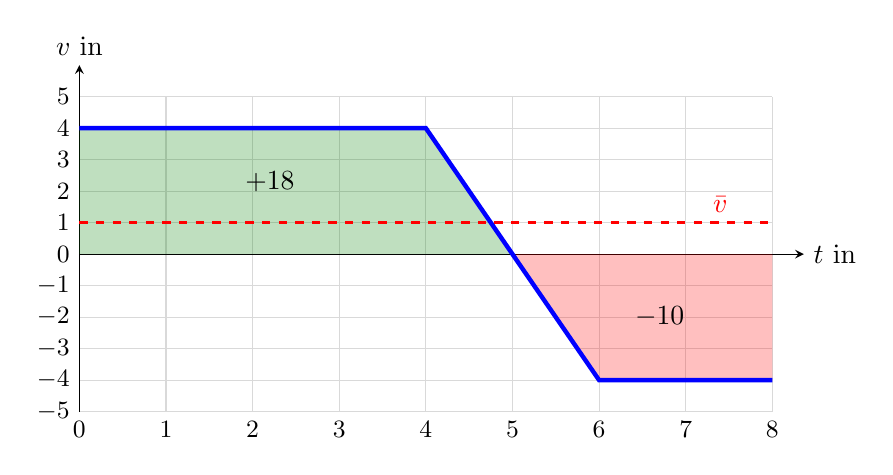
\begin{tikzpicture}[>=stealth, x=1.1cm, y=0.4cm]
 \draw[gray!30] (0,-5) grid[xstep=1, ystep=1] (8,5);
 \draw[->] (0,0) -- (8.364,0) node[right] {$t$ in \si{\second}};
 \draw[->] (0,-5) -- (0,6) node[above] {$v$ in \si{\meter\per\second}};
 \foreach \tk in {0,1,2,3,4,5,6,7,8} \node[below] at (\tk,-5) {\small $\tk$};
 \foreach \yk in {-5,-4,-3,-2,-1,0,1,2,3,4,5} \node[left] at (0,\yk) {\small $\yk$};

 \fill[green!50!black, opacity=0.25] (0,0) -- (0,4) -- (4,4) -- (5,0) -- cycle;
 \fill[red, opacity=0.25] (5,0) -- (6,-4) -- (8,-4) -- (8,0) -- cycle;
 \draw[ultra thick, blue] (0,4) -- (4,4) -- (6,-4) -- (8,-4);
 \draw[very thick, red, dashed] (0,1) -- (8,1);
 \node[above, red] at (7.4,1) {$\bar v$};
 \node at (2.2,2.3) {$+18$};
 \node at (6.7,-2) {$-10$};
\end{tikzpicture}
\end{center}
\abc
\begin{itemize}
\item[(i)] Der Betrag der Geschwindigkeit ist zwar oft \SI{4}{\meter\per\second}, aber am Schluss fährt der Körper rückwärts. Die Strecke rückwärts muss abgezogen werden. $\result{\text{Die Richtung wurde nicht berücksichtigt.}}$
\item[(ii)] \dsP{0}{1} ist die Ortsänderung, keine Geschwindigkeit (falsche Einheit). $\result{\text{Es fehlt die Division durch die Zeit}}$ \tEO.
\item[(iii)] Das Mittel aus Anfangs- und Endgeschwindigkeit ist nur richtig, wenn $v(t)$ eine einzige Gerade ist. $\result{\text{Hier ist } v(t) \text{ keine Gerade}}$: Der Körper fährt \tOneO\ lang vorwärts, aber nur \SI{2}{\second} rückwärts mit \SI{4}{\meter\per\second}.
\end{itemize}
\end{abcliste}
